\newcommand{\inserttreefigure}{
\newcommand{\nodefont}{\scriptsize}
\begin{figure}[t]
\centering
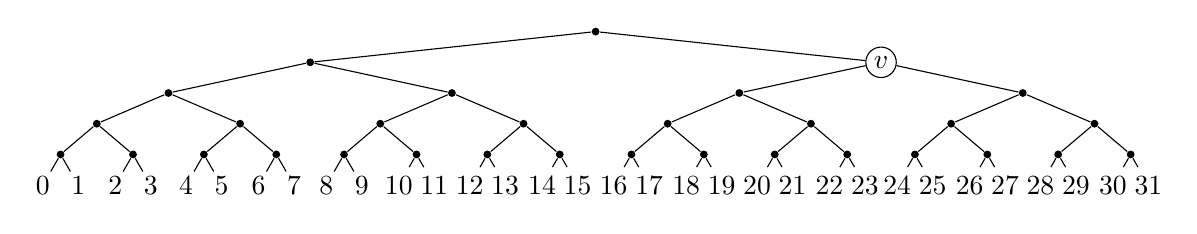
\begin{tikzpicture}[level distance=3.9mm]
\tikzstyle{every node}=[fill=black!100,circle,inner sep=1pt]
\tikzstyle{level 1}=[sibling distance=72.5mm]
\tikzstyle{level 2}=[sibling distance=36mm]
\tikzstyle{level 3}=[sibling distance=18.2mm]
\tikzstyle{level 4}=[sibling distance=9.2mm]
\tikzstyle{level 5}=[sibling distance=4.5mm,set style={{every node}+=[fill=white!15]}]
\node {}
    child {node {}
        child {node {}
            child {node {}
                child {node {}
                    child {node {\nodefont 0}}
                    child {node {\nodefont 1}}
                }
                child {node {}
                    child {node {\nodefont 2}
                    }
                    child {node {\nodefont 3}
                    }
                }
            }
            child {node {}
                child {node {}
                    child {node {\nodefont 4}}
                    child {node {\nodefont 5}}
                }
                child {node {}
                    child {node {\nodefont 6}
                    }
                    child {node {\nodefont 7}
                    }
                }
            }
        }
        child {node {}
            child {node {}
                child {node {}
                    child {node {\nodefont 8}}
                    child {node {\nodefont 9}}
                }
                child {node {}
                    child {node {\nodefont 10}
                    }
                    child {node {\nodefont 11}
                    }
                }
            }
            child {node {}
                child {node {}
                    child {node {\nodefont 12}}
                    child {node {\nodefont 13}}
                }
                child {node {}
                    child {node {\nodefont 14}
                    }
                    child {node {\nodefont 15}
                    }
                }
            }
        }
    }
    child {node[fill=black!00,circle,draw,inner sep=1.5pt] {$v$}
        child {node {}
            child {node {}
                child {node {}
                    child {node {\nodefont 16}}
                    child {node {\nodefont 17}}
                }
                child {node {}
                    child {node {\nodefont 18}
                    }
                    child {node {\nodefont 19}
                    }
                }
            }
            child {node {}
                child {node {}
                    child {node {\nodefont 20}}
                    child {node {\nodefont 21}}
                }
                child {node {}
                    child {node {\nodefont 22}
                    }
                    child {node {\nodefont 23}
                    }
                }
            }
        }
        child {node {}
            child {node {}
                child {node {}
                    child {node {\nodefont 24}}
                    child {node {\nodefont 25}}
                }
                child {node {}
                    child {node {\nodefont 26}
                    }
                    child {node {\nodefont 27}
                    }
                }
            }
            child {node {}
                child {node {}
                    child {node {\nodefont 28}}
                    child {node {\nodefont 29}}
                }
                child {node {}
                    child {node {\nodefont 30}
                    }
                    child {node {\nodefont 31}
                    }
                }
            }
        }
    };
\end{tikzpicture}

%\insertdiagram{tree}
\caption{\label{fig:tree}An information transfer tree $\calT$ with $n=32$ leaves. For the node labelled $v$, the arrival times $t_0=16$, $t_1=23$ and $t_2=31$.}
\end{figure}
}

